\chapter{Contracción muscular y función motora}\label{ch:b2:muscle-movement}

Una velocista sale de los tacos ejerciendo sobre la pista una fuerza de
tres veces su peso, desarrollada en una quinta parte de segundo por unos
músculos que un momento antes estaban relajados. Nada en la célula se ha
acortado para lograrlo: los filamentos de su interior se han deslizado
unos sobre otros, arrastrados por millones de manos moleculares que dan
cada una un paso de diez nanómetros y se sueltan, diez veces por segundo,
pagando un ATP cada vez. Este capítulo toma la \omterm{def:b2:cell-differentiation:myogenesis}{fibra muscular} construida
en el \cref{ch:b2:cell-differentiation} y la pone a trabajar: el
deslizamiento de los filamentos y el motor que los impulsa, el interruptor
de calcio que enciende y apaga el motor, la orden del nervio, la mecánica
de la fuerza y la velocidad, y la manera en que el sistema nervioso gradúa
el conjunto, desde una sacudida hasta un esprint.

\section{Los filamentos deslizantes}

\begin{proposition}[El mecanismo de los filamentos deslizantes]\label{prop:b2:muscle-movement:sliding}
\index{filamentos deslizantes}\index{sarcómero!contracción}
Cuando una \omterm{def:b2:cell-differentiation:myogenesis}{fibra muscular} se acorta, sus \omterm{def:b2:cell-differentiation:fibre}{sarcómeros} se acortan
(\cref{ch:b2:cell-differentiation}), pero ni los filamentos gruesos de
miosina ni los filamentos finos de actina cambian de longitud: los
filamentos finos se deslizan hacia el centro a lo largo de los gruesos, la
banda I y la zona H se estrechan y los discos Z se acercan. La
superposición de los dos conjuntos de filamentos es donde se genera la
fuerza, y un \omterm{def:b2:cell-differentiation:fibre}{sarcómero} genera una fuerza proporcional a esa
superposición: desde una longitud de estiramiento de
\qty{3.6}{\micro m}, sin superposición ni fuerza, la fuerza aumenta
linealmente a medida que los filamentos se superponen más, alcanza una
meseta cerca de \qty{2.2}{\micro m}, donde todas las cabezas de miosina
están frente a la actina, y vuelve a caer por debajo de
\qty{2.0}{\micro m}, cuando los filamentos finos chocan entre sí y los
gruesos tropiezan con los discos Z. La longitud de reposo de un músculo en
el cuerpo se sitúa en la meseta --- que es la primera pista de cómo se
produce la fuerza.
\end{proposition}
\begin{proof}[Evidencia]
A.~F.~Huxley y Niedergerke, y H.~E.~Huxley y Hanson (1954), midieron las
bandas de fibras aisladas y de \omterm{def:b2:cell-differentiation:fibre}{miofibrillas} aisladas mediante microscopía
de interferencia y de contraste de fase mientras se acortaban: la banda A
conservaba su longitud y la banda I se reducía, luego los filamentos se
deslizan. Gordon, Huxley y Julian (1966) mantuvieron una fibra aislada a
longitudes fijas con un dispositivo de retroalimentación que mantenía
constante la longitud de los \omterm{def:b2:cell-differentiation:fibre}{sarcómeros} de un segmento, y hallaron que la
fuerza era proporcional a la superposición de los filamentos gruesos y
finos medida por microscopía electrónica --- la curva longitud--tensión,
con su meseta y sus dos tramos lineales, exactamente como predice la
geometría de los filamentos.
\end{proof}
\begin{omfigure}
\begin{minipage}[b]{0.5\linewidth}\centering
\begin{tikzpicture}[every node/.style={font=\scriptsize}]
  \foreach \y/\lab/\ov in {2.4/{relajado, \qty{2.6}{\micro m}}/0.9, 1.2/{contraído, \qty{2.0}{\micro m}}/0.3} {
    \begin{scope}[yshift=\y cm]
      \draw[very thick, omThm] (0,-0.35) -- (0,0.35); \draw[very thick, omThm] (4.4-2*\ov+1.0,-0.35) -- (4.4-2*\ov+1.0,0.35);
      \pgfmathsetmacro{\len}{4.4-2*\ov+1.0}
      \foreach \dy in {-0.25,0.05,0.25} { \draw[thick, omDef] (0,\dy) -- (1.5,\dy); \draw[thick, omDef] (\len,\dy) -- (\len-1.5,\dy); }
      \draw[line width=3pt, omExo!80!black] (\len/2-1.1,-0.1) -- (\len/2+1.1,-0.1);
      \node[right] at (\len+0.15,0) {\lab};
    \end{scope}
  }
  \node[align=center] at (2.7,0.1) {los filamentos conservan su longitud;\\la superposición crece al acercarse los discos Z};
\end{tikzpicture}
\end{minipage}\hfill
\begin{minipage}[b]{0.48\linewidth}\centering
\begin{tikzpicture}
\begin{axis}[
  width=\linewidth, height=4.8cm,
  axis x line=bottom, axis y line=left,
  xmin=1.2, xmax=3.8, ymin=0, ymax=1.15,
  xlabel={longitud del sarcómero (\unit{\micro m})}, ylabel={fuerza (relativa)},
  xlabel style={font=\scriptsize, at={(axis description cs:0.5,-0.17)}, anchor=north},
  ylabel style={font=\scriptsize},
  tick label style={font=\scriptsize}, xtick={1.3,2.0,2.2,3.6}, ytick={0,0.5,1},
  clip=false,
]
\addplot[very thick, omDef] coordinates {(1.3,0) (1.65,0.5) (2.0,1) (2.2,1) (3.6,0)};
\node[font=\scriptsize, anchor=south] at (axis cs:2.1,1.02) {meseta};
\node[font=\scriptsize, anchor=west, align=left] at (axis cs:2.95,0.75) {superposición\\decreciente};
\end{axis}
\end{tikzpicture}
\end{minipage}

{\small Izquierda: un \omterm{def:b2:cell-differentiation:fibre}{sarcómero} relajado y contraído --- los filamentos
finos (en azul) se deslizan a lo largo de los gruesos (en gris) sin cambiar
de longitud. Derecha: la curva longitud--tensión: la fuerza es
proporcional a la superposición y máxima en la meseta, donde reposa el
músculo.}
\end{omfigure}

\begin{omfigure}
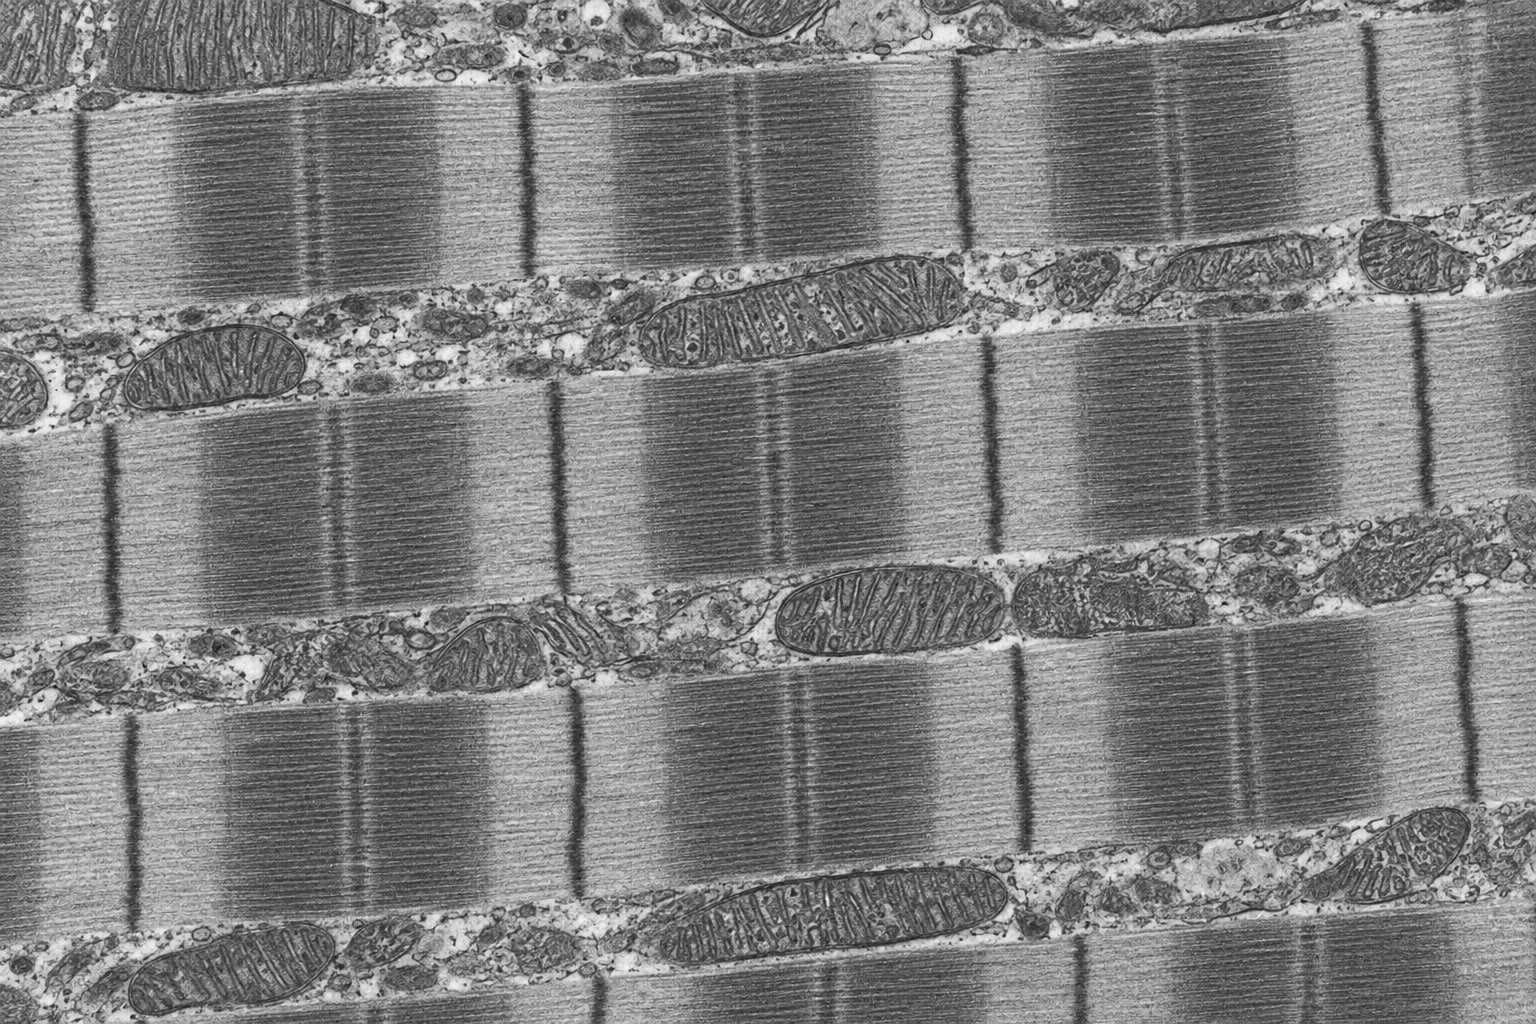
\includegraphics[width=0.6\linewidth]{images/book4/ai/b4-21-sarcomere-tem.jpg}

{\small \omterm{def:b2:cell-differentiation:fibre}{Miofibrillas} al microscopio electrónico: las bandas A de
filamentos gruesos, las bandas I de filamentos finos divididas por las
líneas Z y, entre las fibrillas, las mitocondrias que pagan el
deslizamiento.}
\end{omfigure}

\section{El motor}

\begin{proposition}[El ciclo de los puentes cruzados]\label{prop:b2:muscle-movement:crossbridge}
\index{ciclo de los puentes cruzados}\index{miosina}\index{ATP!en la contracción}
Cada filamento grueso está erizado de unas trescientas \emph{cabezas de
miosina}, y cada cabeza es un motor que camina sobre la actina en un ciclo
de cuatro pasos. (1) Con el ATP unido, la cabeza está separada de la
actina; hidroliza el ATP en ADP y fosfato y se arma en una forma tensa y
de alta energía. (2) La cabeza armada se une a una subunidad de actina y
forma un \emph{puente cruzado}. (3) Se libera el fosfato y la cabeza
recupera bruscamente su forma relajada, arrastrando el filamento fino unos
\qty{10}{nm} hacia el centro del \omterm{def:b2:cell-differentiation:fibre}{sarcómero} --- el \emph{golpe de fuerza};
el ADP sale. (4) Un nuevo ATP se une y la cabeza suelta la actina; sin ATP
no puede soltarse, y esa es la rigidez de la muerte. El ciclo dura
alrededor de una vigésima de segundo; una cabeza pasa la mayor parte de él
separada, de modo que en cada instante solo tira una fracción de las
cabezas, y un filamento que se desliza deprisa nunca queda suelto.
La fuerza es la suma de los tirones de las cabezas unidas; el acortamiento,
la suma de sus pasos, como máximo medio micrómetro por \omterm{def:b2:cell-differentiation:fibre}{sarcómero} por ciclo;
y la energía es un ATP por paso por cabeza, unos
\qty{50}{kJ/mol} --- \qty{8e-20}{J} por paso, de los que la cabeza
convierte hasta la mitad en trabajo.
\end{proposition}

\begin{omfigure}
\begin{tikzpicture}[every node/.style={font=\scriptsize}, >=stealth]
  \foreach \x/\lab/\ang/\att in {0/{1. ATP unido:\\cabeza separada;\\ATP hidrolizado,\\cabeza armada}/60/0, 3.6/{2. la cabeza armada\\se une a la actina:\\puente cruzado}/60/1, 7.2/{3. sale el fosfato:\\golpe de fuerza,\\filamento desplazado\\\qty{10}{nm}}/20/1, 10.8/{4. sale el ADP, se une\\un ATP nuevo:\\la cabeza se suelta}/20/0} {
    \begin{scope}[xshift=\x cm]
      \draw[thick, omDef] (0,2.2) -- (2.8,2.2); \foreach \i in {0.2,0.6,...,2.6} \fill[omDef!50] (\i,2.2) circle (0.14);
      \draw[line width=3pt, omExo!80!black] (0,0.4) -- (2.8,0.4);
      \draw[very thick, omThm] (1.4,0.4) -- (1.4,1.0);
      \ifnum\att=1 \draw[very thick, omThm] (1.4,1.0) -- ++(\ang:1.15); \fill[omThm] (1.4,1.0) ++(\ang:1.15) circle (0.16); \else \draw[very thick, omThm] (1.4,1.0) -- ++(\ang:1.0); \fill[omThm] (1.4,1.0) ++(\ang:1.0) circle (0.16); \fi
      \node[below, align=center] at (1.4,0.15) {\lab};
    \end{scope}
  }
  \draw[->, thick, omDef] (7.9,2.55) -- (8.9,2.55); \node[omDef, above] at (8.4,2.6) {el filamento fino avanza};
\end{tikzpicture}

{\small El \omterm{prop:b2:muscle-movement:crossbridge}{ciclo de los puentes cruzados}. Una cabeza de miosina armada (en
rojo) se une a la actina (en azul), libera el fosfato y arrastra el
filamento fino con su golpe de fuerza; después une un ATP nuevo y se
suelta.}
\end{omfigure}

\begin{theorem}[Fuerza, velocidad y potencia de un músculo]\label{thm:b2:muscle-movement:hill}
\index{curva fuerza--velocidad}\index{potencia muscular}
La fuerza de un músculo disminuye cuanto más deprisa se acorta, porque
cuanto más rápido se deslizan los filamentos, menos cabezas están unidas
en cada instante y más de ellas son arrastradas más allá de su golpe antes
de soltarse. La relación de Hill lo describe:
\[
(F + a)(v + b) = (F_0 + a)\,b,
\]
donde $F_0$ es la fuerza isométrica (con $v = 0$), $v_{\max} =
F_0 b/a$ la velocidad sin carga, y $a$, $b$ constantes ($a \approx
F_0/4$). La potencia $Fv$ es nula en ambos extremos y máxima hacia un
tercio de $v_{\max}$ y un tercio de $F_0$ --- por eso un ciclista cambia
de marcha y la zancada de un velocista tiene una frecuencia preferida. Un
músculo humano desarrolla unos \qty{30}{N} por centímetro cuadrado de
sección, se acorta a hasta diez longitudes por segundo y proporciona, en
su punto óptimo, unos \qty{100}{W} por kilogramo.
\end{theorem}
\begin{proof}
La curva de Hill es empírica (1938), medida en músculo aislado de rana
como la velocidad de acortamiento frente a la carga que levanta; la
hipérbola se ajusta porque la fracción de cabezas unidas disminuye con la
velocidad de deslizamiento y la fuerza de cada cabeza unida disminuye a
medida que es arrastrada a lo largo de su golpe. Potencia: con
$F = (F_0 + a)b/(v + b) - a$, $Fv$ es nula en
$v = 0$ y en $v_{\max}$; derivando se obtiene el máximo en
$v = b(\sqrt{(F_0 + a)/a} - 1)$, que para $a = F_0/4$ es $v =
1.24\,b = 0.31\,v_{\max}$, donde $F = 0.31\,F_0$.
\end{proof}

\begin{omfigure}
\begin{tikzpicture}
\begin{axis}[
  width=0.7\linewidth, height=5.4cm,
  axis x line=bottom, axis y line=left,
  xmin=0, xmax=1.05, ymin=0, ymax=1.1,
  xlabel={velocidad de acortamiento $v/v_{\max}$}, ylabel={fuerza $F/F_0$, potencia (relativa)},
  xlabel style={font=\small, at={(axis description cs:0.5,-0.13)}, anchor=north},
  ylabel style={font=\small},
  tick label style={font=\small}, xtick={0,0.31,1}, xticklabels={0,0.31,1}, ytick={0,0.31,1}, yticklabels={0,0.31,1},
  legend style={font=\scriptsize, at={(0.97,0.95)}, anchor=north east, draw=none},
  clip=false,
]
\addplot[very thick, omDef, domain=0:1, samples=100] {(1.25*0.25)/(x+0.25) - 0.25};
\addlegendentry{fuerza}
\addplot[very thick, omThm, domain=0:1, samples=100] {10.4*x*((1.25*0.25)/(x+0.25) - 0.25)};
\addlegendentry{potencia (a escala)}
\draw[dashed, gray] (axis cs:0.31,0) -- (axis cs:0.31,1.0);
\end{axis}
\end{tikzpicture}

{\small La \omterm{thm:b2:muscle-movement:hill}{curva fuerza--velocidad} de Hill ($a = F_0/4$) y la potencia que
implica: la fuerza disminuye cuanto más deprisa se acorta el músculo, y la
potencia es máxima hacia un tercio de la velocidad máxima y un tercio de la
fuerza isométrica.}
\end{omfigure}

\section{El interruptor: el calcio}

\begin{proposition}[Acoplamiento excitación--contracción]\label{prop:b2:muscle-movement:coupling}
\index{acoplamiento excitación--contracción}\index{troponina}\index{tropomiosina}\index{retículo sarcoplásmico}
En reposo, las cabezas de miosina no pueden alcanzar la actina: los sitios
de unión del filamento fino están cubiertos por la \emph{tropomiosina},
una varilla alojada en el surco de la hélice de actina y mantenida allí
por la \emph{troponina}. El interruptor es el calcio. Un \omterm{prop:b2:neurons-synapses:ap}{potencial de
acción} en la membrana de la fibra desciende por los \omterm{def:b2:cell-differentiation:fibre}{túbulos T} hacia el
interior y, en las uniones donde un \omterm{def:b2:cell-differentiation:fibre}{túbulo T} se encuentra con el \omterm{def:b2:cell-differentiation:fibre}{retículo
sarcoplásmico}, abre los canales de liberación de calcio del retículo; el
calcio inunda las \omterm{def:b2:cell-differentiation:fibre}{miofibrillas}, sube de \qty{0.1}{} a
\qty{10}{\micro mol/L} en un milisegundo, se une a la troponina, y la
troponina desplaza la tropomiosina fuera de los sitios de unión: las
cabezas se unen y la fibra se contrae mientras el calcio permanezca. Unas
bombas del retículo, que consumen ATP, recuperan el calcio en unas decenas
de milisegundos; la tropomiosina vuelve a cubrir los sitios y la fibra se
relaja. La relajación es, por tanto, tan activa como la contracción, y un
músculo privado de ATP no puede ni soltar sus cabezas ni bombear su
calcio --- la rigidez cadavérica. En el \omterm{def:b2:heart:anatomy}{corazón} se usa el mismo
interruptor, pero con calcio que entra desde el exterior por los propios
canales de la membrana para desencadenar la liberación, y por eso el
\omterm{def:b2:heart:anatomy}{corazón}, y no el músculo esquelético, es sensible al calcio de la
\omterm{def:b2:blood-circulation:blood}{sangre}.
\end{proposition}
\begin{omfigure}
\begin{tikzpicture}[every node/.style={font=\scriptsize}, >=stealth]
  \node[draw, rounded corners, fill=omDef!15, align=center] (nerve) at (0,0) {impulso del\\nervio motor};
  \node[draw, rounded corners, fill=omDef!15, align=center] (nmj) at (3.0,0) {unión\\neuromuscular:\\acetilcolina};
  \node[draw, rounded corners, fill=omDef!15, align=center] (ap) at (6.2,0) {potencial de acción\\muscular, por\\los túbulos T};
  \node[draw, rounded corners, fill=omThm!15, align=center] (ca) at (9.4,0) {liberación de Ca$^{2+}$\\desde el retículo\\sarcoplásmico};
  \node[draw, rounded corners, fill=omProp!20, align=center] (tn) at (12.6,0) {la troponina une Ca$^{2+}$,\\la tropomiosina se mueve,\\las cabezas se unen};
  \node[draw, rounded corners, fill=omExo!25, align=center] (off) at (9.4,-2.2) {las bombas recuperan el Ca$^{2+}$ (ATP);\\la tropomiosina cubre la actina:\\relajación};
  \draw[->, thick] (nerve) -- (nmj); \draw[->, thick] (nmj) -- (ap); \draw[->, thick] (ap) -- (ca); \draw[->, thick] (ca) -- (tn);
  \draw[->, thick] (ca) -- (off);
  \node[below, gray] at (1.5,-0.7) {\qty{0.6}{ms}}; \node[below, gray] at (4.6,-0.7) {\qty{1}{ms}}; \node[below, gray] at (7.8,-0.7) {\qty{1}{ms}};
\end{tikzpicture}

{\small Del impulso nervioso a la fuerza: la unión, el \omterm{prop:b2:neurons-synapses:ap}{potencial de acción}
propio de la fibra, la liberación de calcio y el descubrimiento de los
sitios de la actina --- y después las bombas que lo terminan.}
\end{omfigure}

\section{La orden y la graduación}

\begin{definition}[La unidad motora]\label{def:b2:muscle-movement:motorunit}
\index{unidad motora}\index{sacudida muscular}\index{tétanos}\index{reclutamiento}
Una \emph{motoneurona} de la médula espinal envía su \omterm{def:b2:neurons-synapses:neuron}{axón} a un músculo y
se ramifica para inervar desde unas pocas hasta mil fibras, dispersas por
el músculo; la \omterm{def:b2:neurons-synapses:neuron}{neurona} y sus fibras forman una \emph{unidad motora}, la
menor cantidad de fuerza que el sistema nervioso puede ordenar. Cada
impulso de la \omterm{def:b2:neurons-synapses:neuron}{neurona} hace que todas las fibras de la unidad disparen una
vez y den una \emph{sacudida}: una fuerza que sube en unos \qty{30}{ms} y
decae en \qty{100}{ms}, porque el pulso de calcio es breve. Los impulsos
en rápida sucesión hacen que las sacudidas se sumen, puesto que el calcio
de una no se ha bombeado todavía cuando llega la siguiente; a unos 30
a 50 impulsos por segundo, la fuerza se fusiona en un \emph{tétanos} liso,
de tres a cinco veces la sacudida. El sistema nervioso gradúa la fuerza de
un músculo de dos maneras: por la \emph{frecuencia} con la que dispara cada
unidad y por el \emph{número} de unidades que recluta --- primero las
pequeñas, lentas y resistentes a la fatiga (el \emph{principio del
tamaño}), y al final las grandes y rápidas, solo para los mayores
esfuerzos. Un músculo en uso corriente nunca está, por tanto, activado del
todo: una fracción de sus unidades dispara, por turnos, y el resto
descansa.
\end{definition}

\begin{omfigure}
\begin{tikzpicture}
\begin{axis}[
  width=0.82\linewidth, height=5.4cm,
  axis x line=bottom, axis y line=left,
  xmin=0, xmax=1.0, ymin=0, ymax=4.2,
  xlabel={tiempo (s)}, ylabel={fuerza (sacudida $=$ 1)},
  xlabel style={font=\small, at={(axis description cs:0.5,-0.13)}, anchor=north},
  ylabel style={font=\small},
  tick label style={font=\small}, xtick={0,0.2,0.4,0.6,0.8,1}, ytick={0,1,2,3,4},
  clip=false,
]
% single twitch
\addplot[very thick, omDef, domain=0:0.2, samples=60] {(x<0.02)*0 + (x>=0.02)*4.5*(x-0.02)*exp(-(x-0.02)/0.03)*4.1};
% summation at 10 Hz
\addplot[very thick, omProp, domain=0.25:0.62, samples=200] {(x>=0.25)*4.5*4.1*(x-0.25)*exp(-(x-0.25)/0.03) + (x>=0.33)*4.5*4.1*(x-0.33)*exp(-(x-0.33)/0.03) + (x>=0.41)*4.5*4.1*(x-0.41)*exp(-(x-0.41)/0.03) + (x>=0.49)*4.5*4.1*(x-0.49)*exp(-(x-0.49)/0.03)};
% tetanus at 50 Hz
\addplot[very thick, omThm, domain=0.66:0.98, samples=100] {3.8*(1-exp(-(x-0.66)/0.06))};
\node[font=\scriptsize, anchor=west] at (axis cs:0.09,0.7) {un impulso: sacudida};
\node[font=\scriptsize, anchor=south] at (axis cs:0.44,2.2) {\qty{12}{Hz}: suma};
\node[font=\scriptsize, anchor=south] at (axis cs:0.82,3.85) {\qty{50}{Hz}: tétanos fusionado};
\end{axis}
\end{tikzpicture}

{\small Graduar la fuerza mediante la frecuencia. Un solo impulso da una
sacudida; los impulsos a una docena por segundo se suman en una fuerza
ondulante; a cincuenta por segundo, la fuerza se fusiona en un \omterm{def:b2:muscle-movement:motorunit}{tétanos} de
varias veces la sacudida.}
\end{omfigure}

\begin{proposition}[Los reflejos y la médula espinal]\label{prop:b2:muscle-movement:reflex}
\index{arco reflejo}\index{huso muscular}\index{reflejo miotático}\index{inhibición recíproca}
La motoneurona es la \emph{vía final común}: toda orden, venga de la
corteza o de un reflejo, termina en ella. El circuito más sencillo es el
\emph{\omterm{prop:b2:muscle-movement:reflex}{reflejo miotático}} del \cref{ch:b2:neurons-synapses}: unas
terminaciones sensitivas enrolladas alrededor de fibras especiales situadas
dentro del músculo, los \emph{\omterm{prop:b2:muscle-movement:reflex}{husos musculares}}, descargan cuando el
músculo se estira, excitan las motoneuronas del mismo músculo a través de
una \omterm{def:b2:neurons-synapses:synapse}{sinapsis} e inhiben las del antagonista a través de una interneurona
(\emph{\omterm{prop:b2:muscle-movement:reflex}{inhibición recíproca}}), de modo que el músculo se opone al
estiramiento --- la base de la postura, puesto que cada balanceo estira
algún músculo. Un segundo receptor, el órgano tendinoso, descarga cuando
la fuerza del músculo es alta e inhibe sus propias motoneuronas: una
válvula de seguridad. La retirada ante un estímulo doloroso es un reflejo
de varias \omterm{def:b2:neurons-synapses:synapse}{sinapsis} que flexiona el miembro y, en el otro lado, extiende el
miembro opuesto para no caer. Y el encéfalo no ordena músculos sino
movimientos: la corteza envía un plan, el cerebelo lo corrige según lo que
informan los husos, los ganglios basales lo liberan, y los circuitos de la
médula espinal, que pueden generar por sí solos un ritmo de marcha, lo
ejecutan --- el tema del volumen del tercer año.
\end{proposition}

\begin{omfigure}
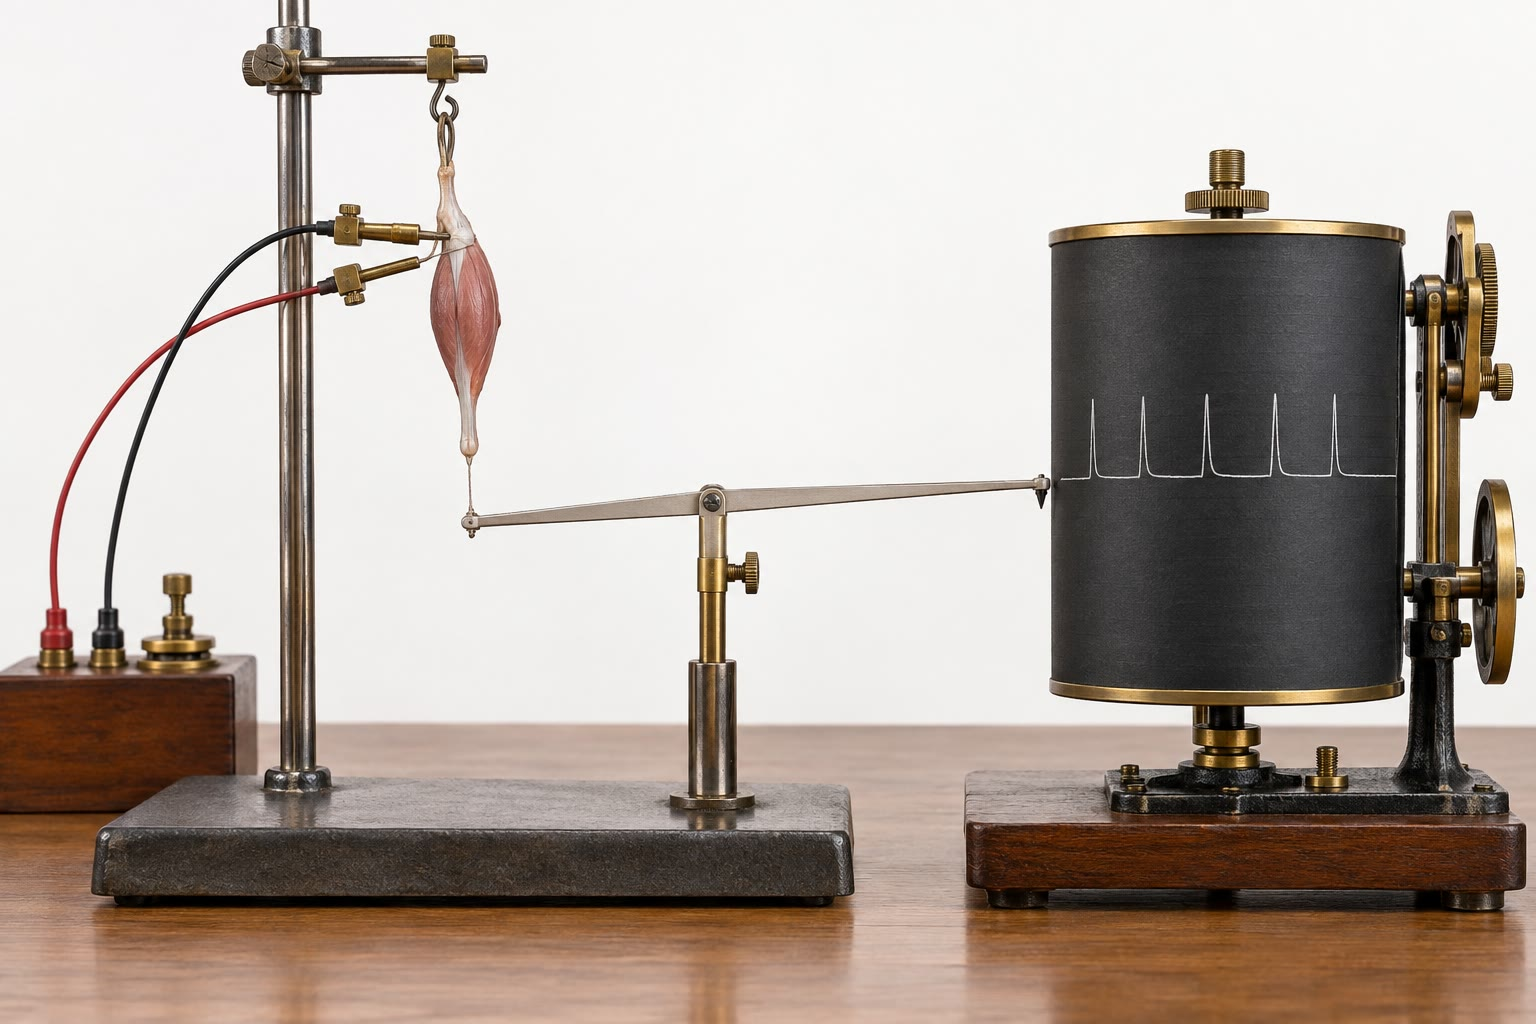
\includegraphics[width=0.44\linewidth]{images/book4/ai/b4-21-frog-muscle-prep.jpg}\hspace{0.04\linewidth}
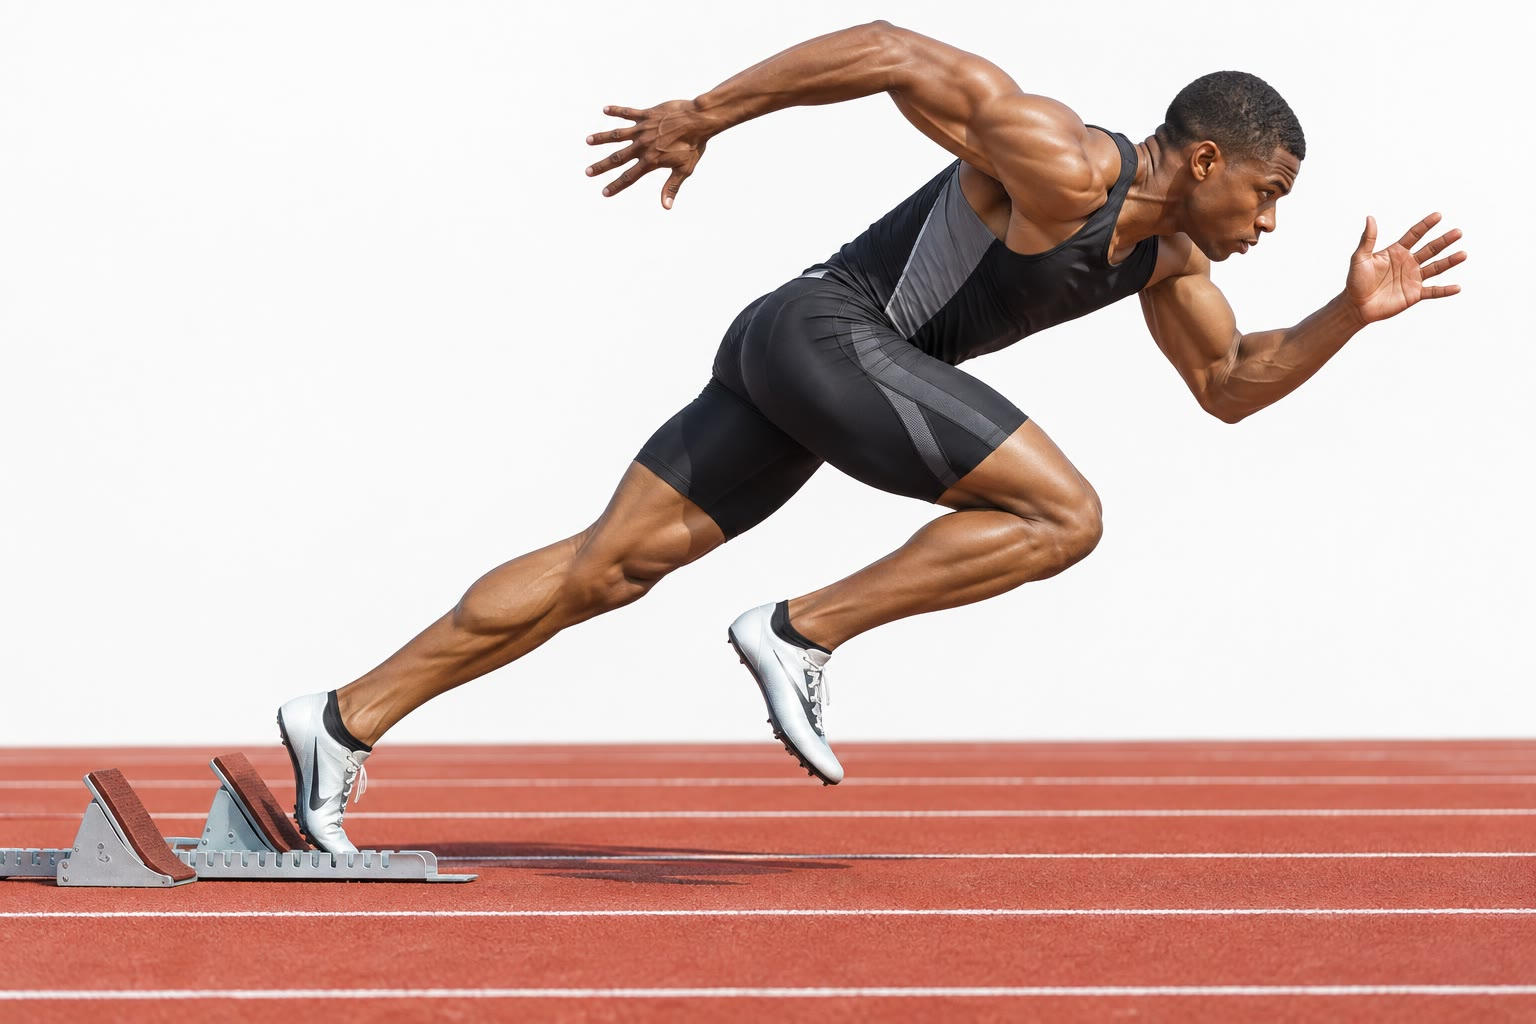
\includegraphics[width=0.44\linewidth]{images/book4/ai/b4-21-sprinter.jpg}

{\small Izquierda: la preparación clásica --- un músculo de rana, su
nervio, unos electrodos de estimulación y una palanca que escribe sobre un
tambor ahumado ---, en la que se registraron por primera vez la sacudida,
la suma y el \omterm{def:b2:muscle-movement:motorunit}{tétanos}. Derecha: la misma fisiología a pleno rendimiento.}
\end{omfigure}

\section{Combustible y fatiga}

\begin{proposition}[Pagar el trabajo]\label{prop:b2:muscle-movement:energy}
\index{fosfocreatina}\index{fatiga muscular}\index{deuda de oxígeno}
Una fibra contiene ATP para uno o dos segundos de esfuerzo máximo. La
primera reserva es la \emph{fosfocreatina}, que refosforila el ADP en
milisegundos y dura unos diez segundos --- el combustible del velocista.
La segunda es la \emph{glucólisis} del glucógeno de la fibra, sin oxígeno,
que rinde dos ATP por glucosa y lactato: rápida, suficiente para uno o dos
minutos, y autolimitada a medida que se acumulan ácido y fosfato. La
tercera es el metabolismo \emph{oxidativo} de la glucosa y los ácidos
grasos en las mitocondrias, treinta ATP por glucosa, limitado solo por el
oxígeno que aporta la \omterm{def:b2:blood-circulation:blood}{sangre}
(\cref{ch:b2:blood-pressure}): el maratón. Las fibras rápidas glucolíticas
dependen de las dos primeras y se cansan en un minuto; las fibras lentas
oxidativas, rojas por la mioglobina y repletas de mitocondrias, funcionan
durante horas. La \emph{fatiga} en un esfuerzo corto no es el agotamiento
del ATP --- que dejaría el músculo rígido ---, sino la acumulación de
fosfato y de protones, que debilitan los puentes cruzados y la liberación
de calcio; en un esfuerzo largo es el agotamiento del glucógeno y, al
final, de la voluntad. Tras el esfuerzo, el músculo paga su \emph{\omterm{prop:b2:muscle-movement:energy}{deuda de
oxígeno}}: restablece la fosfocreatina, reconvierte el lactato (en el
hígado) y rellena sus reservas, y se sigue respirando con fuerza durante
minutos después de detenerse.
\end{proposition}

\begin{example}[Cien metros]\label{ex:b2:muscle-movement:sprint}
Diez segundos de esfuerzo máximo de \qty{20}{kg} de músculo de las piernas
a \qty{100}{W/kg} son \qty{2}{kW} de potencia mecánica y, con un
rendimiento del \qty{25}{\%}, \qty{8}{kW} de recambio de ATP --- unos
\qty{160}{mmol} de ATP por segundo, o unos \qty{800}{g} de ATP en la
carrera. El músculo contiene unos cincuenta gramos; la fosfocreatina cubre los
cinco primeros segundos y la glucólisis el resto, y la velocista termina
con \qty{15}{mmol/L} de lactato en la \omterm{def:b2:blood-circulation:blood}{sangre} y una deuda que paga durante
el cuarto de hora siguiente. Una maratoniana a \qty{300}{W} durante dos
horas consume \qty{2}{MJ} de trabajo, \qty{8}{MJ} de combustible --- un
kilogramo de glucógeno y grasa ---, con un aporte de oxígeno de
\qty{4}{L/min} durante todo el recorrido, y el muro con el que choca hacia
el kilómetro treinta es el fondo de sus reservas de glucógeno.
\end{example}

\section{Ejercicios}

\begin{exercise}[$\star$]\label{exo:b2:muscle-movement:1}
Enúnciese el mecanismo de los \omterm{prop:b2:muscle-movement:sliding}{filamentos deslizantes} e indíquese qué
bandas del \omterm{def:b2:cell-differentiation:fibre}{sarcómero} cambian durante la contracción y cuáles no.
\end{exercise}

\begin{exercise}[$\star$]\label{exo:b2:muscle-movement:2}
Dense los cuatro pasos del \omterm{prop:b2:muscle-movement:crossbridge}{ciclo de los puentes cruzados} y el papel del
ATP en cada uno. ¿Por qué se pone rígido un músculo sin ATP?
\end{exercise}

\begin{exercise}[$\star$]\label{exo:b2:muscle-movement:3}
Enumérense los sucesos que van del impulso de un nervio motor a la unión de
las cabezas de miosina, con el tiempo que lleva cada uno.
\end{exercise}

\begin{exercise}[$\star$]\label{exo:b2:muscle-movement:4}
Defínanse \omterm{def:b2:muscle-movement:motorunit}{unidad motora}, sacudida y \omterm{def:b2:muscle-movement:motorunit}{tétanos}, y dense las dos maneras en
que el sistema nervioso gradúa la fuerza.
\end{exercise}

\begin{exercise}[$\star\star$]\label{exo:b2:muscle-movement:5}
Un \omterm{def:b2:cell-differentiation:fibre}{sarcómero} de \qty{2.4}{\micro m} se acorta a \qty{2.0}{\micro m} en
\qty{50}{ms}. Calcúlense la velocidad de deslizamiento de los filamentos
finos respecto de los gruesos y, con un paso de \qty{10}{nm}, el número de
ciclos que debe realizar por segundo cada cabeza unida.
\end{exercise}

\begin{exercise}[$\star\star$]\label{exo:b2:muscle-movement:6}
Una fibra de \qty{10}{cm} tiene \num{40000} \omterm{def:b2:cell-differentiation:fibre}{sarcómeros} en serie y se acorta
un \qty{20}{\%} en \qty{0.1}{s}. Calcúlense su velocidad de acortamiento en
longitudes por segundo y en metros por segundo, y la velocidad de cada
\omterm{def:b2:cell-differentiation:fibre}{sarcómero}.
\end{exercise}

\begin{exercise}[$\star\star$]\label{exo:b2:muscle-movement:7}
Con la relación de Hill y $a = F_0/4$, $v_{\max} = 10$ longitudes por
segundo, calcúlense la fuerza (como fracción de $F_0$) a 1, 3 y 6
longitudes por segundo, y la potencia en cada caso. ¿Dónde es máxima la
potencia?
\end{exercise}

\begin{exercise}[$\star\star$]\label{exo:b2:muscle-movement:8}
Un cuádriceps de \qty{80}{cm^2} de sección a \qty{30}{N/cm^2}: calcúlese su
fuerza isométrica máxima. Actúa a \qty{5}{cm} de la articulación de la
rodilla sobre una palanca cuyo pie está a \qty{45}{cm} de la articulación:
¿qué fuerza puede ejercer el pie?
\end{exercise}

\begin{exercise}[$\star\star$]\label{exo:b2:muscle-movement:9}
El pulso de calcio de una sacudida dura \qty{30}{ms}. Explíquese por qué
los impulsos a \qty{10}{Hz} dan una fuerza ondulante y a \qty{50}{Hz} un
\omterm{def:b2:muscle-movement:motorunit}{tétanos} liso, y por qué la fuerza tetánica supera la de la sacudida.
\end{exercise}

\begin{exercise}[$\star\star\star$]\label{exo:b2:muscle-movement:10}
Los \qty{20}{kg} de músculo de las piernas de una velocista proporcionan
\qty{2}{kW} durante \qty{10}{s} con un rendimiento del \qty{25}{\%}.
Calcúlense el ATP utilizado (\qty{50}{kJ/mol}), la fosfocreatina necesaria
para cubrir los \qty{5}{s} primeros y la glucosa fermentada para cubrir el
resto (2 ATP por glucosa). ¿Qué concentración de lactato supone eso en
\qty{40}{L} de agua corporal?
\end{exercise}

\begin{exercise}[$\star\star\star$]\label{exo:b2:muscle-movement:11}
Predígase el efecto sobre la contracción de: un fármaco que bloquea el
canal de liberación de calcio del retículo; otro que bloquea su bomba; una
\omterm{def:b2:genome-diversification:mutation}{mutación} que hace la troponina insensible al calcio; la eliminación del
calcio de la \omterm{def:b2:blood-circulation:blood}{sangre}, para el músculo esquelético y para el \omterm{def:b2:heart:anatomy}{corazón}.
\end{exercise}

\begin{exercise}[$\star\star\star$]\label{exo:b2:muscle-movement:12}
``Un músculo es una máquina que convierte energía química en fuerza con el
rendimiento de un buen motor y el control de un ordenador.'' Discútanse el
rendimiento (de un cuarto a la mitad), lo que lo limita, y lo que aportan
las dos maneras de graduar la fuerza del sistema nervioso que no aportaría
un simple interruptor.
\end{exercise}

\section{Problema: la fisiología de un salto}

\begin{problem}[{Problema de fin de semana --- un salto a pies juntos
analizado desde el sarcómero hasta el despegue: el deslizamiento, los
puentes cruzados, el interruptor de calcio, el límite fuerza--velocidad,
las unidades motoras y el combustible, hasta llegar al número de golpes de
los puentes cruzados, la fuerza a la velocidad de despegue y el ATP que
cuesta el salto}]
\label{pb:b2:muscle-movement:1}
Una persona de \qty{70}{kg} salta \qty{40}{cm} en vertical, elevando el
centro de masas del cuerpo \qty{0.4}{m} durante un empuje de
\qty{0.3}{s}. Los extensores de la pierna (\qty{20}{kg} de músculo) tienen
una sección conjunta de \qty{500}{cm^2} a \qty{30}{N/cm^2}; sus fibras
miden \qty{12}{cm} (\num{48000} \omterm{def:b2:cell-differentiation:fibre}{sarcómeros}) y se acortan \qty{4}{cm}
durante el empuje; las articulaciones multiplican el acortamiento del
músculo por \num{10} en el pie y dividen su fuerza por el mismo factor.
$v_{\max} = 8$ longitudes por segundo, $a = F_0/4$. Cada filamento grueso
porta \num{300} cabezas de miosina; hay $6\times
10^{10}$ filamentos gruesos por centímetro cuadrado de músculo; un golpe
mide \qty{10}{nm} y cuesta un ATP (\qty{8e-20}{J}, \qty{50}{kJ/mol});
rendimiento del \qty{40}{\%}. El músculo contiene \qty{5}{mmol/kg} de ATP
y \qty{20}{mmol/kg} de fosfocreatina. Las fibras miden \qty{60}{\micro
m} de diámetro. \omterm{def:b2:muscle-movement:motorunit}{Unidades motoras}: \num{800} por grupo muscular, de
\num{50} a \num{2000} fibras cada una.

\medskip
\noindent\textbf{Parte I --- La mecánica.}
\begin{enumerate}
  \item Calcúlense la velocidad de despegue necesaria para elevarse
        \qty{40}{cm} ($v^{2} = 2gh$) y la energía cinética en el despegue.
  \item Calcúlese la fuerza media que ejercen las piernas sobre el suelo
        durante el empuje (el trabajo sobre \qty{0.4}{m} es igual a la
        energía cinética más el trabajo contra la gravedad), y compárese
        con el peso.
  \item Calcúlense la fuerza isométrica máxima de los extensores y, con la
        relación de palanca de 10, la fuerza máxima que podría dar en el
        pie.
  \item Calcúlese la velocidad de acortamiento de las fibras en longitudes
        por segundo y como fracción de $v_{\max}$.
  \item Con la relación de Hill, calcúlense la fuerza disponible a esa
        velocidad como fracción de $F_0$ y la fuerza que da en el pie.
        ¿Puede el músculo solo realizar el salto? ¿De dónde procede el
        resto?
  \item Calcúlense la potencia mecánica media durante el empuje y la
        potencia por kilogramo de extensor.
\end{enumerate}

\medskip
\noindent\textbf{Parte II --- Los puentes cruzados.}
\begin{enumerate}[resume]
  \item ¿Cuánto se acorta cada \omterm{def:b2:cell-differentiation:fibre}{sarcómero}, y cuántos golpes de
        \qty{10}{nm} deben darse a lo largo de cada hemisarcómero para
        deslizar sus filamentos esa distancia?
  \item Calcúlense la velocidad de deslizamiento en cada hemisarcómero y el
        número de golpes por segundo que daría una cabeza si estuviera
        unida de forma continua.
  \item Calcúlese el número de cabezas de miosina de los extensores.
  \item Calcúlense el trabajo que realiza el propio músculo (su fuerza a la
        velocidad del salto por su acortamiento), el trabajo por golpe con
        un rendimiento del \qty{40}{\%} y el número de golpes necesarios.
  \item ¿Cuántos golpes supone eso por cabeza, frente al número disponible
        según la pregunta 7? Coméntese la reserva.
  \item Calcúlese el ATP consumido por el salto, en moles y en gramos
        (\qty{507}{g/mol}), y compruébese el rendimiento a partir de la
        energía de ese ATP.
\end{enumerate}

\medskip
\noindent\textbf{Parte III --- El interruptor y la orden.}
\begin{enumerate}[resume]
  \item El empuje dura \qty{0.3}{s} y el pulso de calcio de un impulso,
        \qty{30}{ms}. ¿Qué frecuencia de disparo mantiene las
        fibras en \omterm{def:b2:muscle-movement:motorunit}{tétanos}, y cuántos impulsos envía cada motoneurona?
  \item El calcio libre sube de \qty{0.1}{} a \qty{10}{\micro
        mol/L} en una fibra de \qty{5e-10}{L}. ¿Cuántos iones de calcio
        libre son, y cuántos ciclos de bomba (dos iones por ATP) cuesta
        recuperarlos?
  \item Calcúlense el número de fibras de los extensores y el ATP de los
        puentes cruzados por fibra y por impulso, y compárese con el coste
        de bombeo de la pregunta 14. El coste real del bombeo es de
        alrededor de una cuarta parte del ATP del músculo: ¿qué subestima
        el calcio libre?
  \item El sistema nervioso recluta las unidades por tamaño. Para el salto,
        ¿qué unidades se reclutan y en qué orden? ¿Qué fracción de las
        \num{800} usaría un paso suave?
  \item Explíquese por qué la fuerza puede graduarse con precisión en los
        esfuerzos pequeños y solo de forma burda cerca del máximo.
  \item Una persona tratada con un fármaco que bloquea la \omterm{prop:b2:neurons-synapses:integration}{unión
        neuromuscular} a medias: predíganse la sacudida, el \omterm{def:b2:muscle-movement:motorunit}{tétanos} y el
        salto.
\end{enumerate}

\medskip
\noindent\textbf{Parte IV --- El combustible.}
\begin{enumerate}[resume]
  \item Calcúlese el ATP almacenado en los extensores y compárese con el
        consumo del salto.
  \item Calcúlense la reserva de fosfocreatina y el número de saltos que
        podría pagar.
  \item Diez saltos seguidos: ¿qué combustible toma el relevo, y qué se
        acumula?
  \item La \omterm{def:b2:blood-circulation:blood}{sangre} puede aportar \qty{2}{L} de oxígeno por minuto a los
        extensores (6 ATP por $\mathrm{O_2}$). ¿Qué recambio de ATP exige
        la potencia del salto, y qué aporte de oxígeno supondría?
        Conclúyase.
  \item Tras los saltos, la persona respira con fuerza durante un minuto.
        Calcúlese el oxígeno necesario para resintetizar la fosfocreatina
        y el ATP utilizados (\qty{6}{ATP} por molécula de
        $\mathrm{O_2}$) y compárese con el consumo en reposo de
        \qty{250}{mL/min}.
  \item ¿Por qué el músculo de un saltador no entra en rigidez aunque el
        ATP se recambie a semejante ritmo?
  \item Enúnciese el resultado: los golpes por hemisarcómero, la fracción
        de fuerza a la velocidad del salto y el ATP que cuesta el salto.
\end{enumerate}
\end{problem}
